\section{Definizione dell'intervento di sistemazione e trasporto solido atteso}
Al fine di dimensionare le opere idrauliche da poter costruire all'interno del bacino idraulico, è necessario studiare le caratteristiche morfologiche del bacino stesso e del reticolo idraulico che lo attraversa.\\
Infatti, il processo erosivo prodotto dal reticolo idraulico dipende da:
\begin{itemize}
    \item tipologia del corso d'acqua alluvionale ed i suoi gradi di libertà (incisione ed allargamento);
    \item forma di trasporto solido prevalente: di fondo, iperconcentrato, colate detritiche,...;
    \item tipo di torrente: di scavo o di trasporto.
\end{itemize}
Il trasporto solido generato dalla corrente può essere:
\begin{itemize}
    \item ``bedload" (di fondo): comprende lo strisciamento, rotolamento o saltellamento dei sedimenti del letto del fiume;
    \item ``suspended load" (in sospensione): è generato dai vortici di turbolenza del flusso d'acqua, e trasporta generalmente il materiale di piccole dimensioni.
\end{itemize} 
\subsubsection{Equilibrio e dinamica del torrente}
Le modificazioni che si verificano in un corso d'acqua sono il risultato della sua tendenza a trovare uno stato di equilibrio.\\
Questo concetto può essere compreso considerando la ``Bilancia di Lane" (1955), ovvero una rappresentazione grafica che permette di capire come sarà il comportamento di un corso d'acqua al fine di raggiungere il proprio equilibrio.
\begin{figure}[H]  \centering
    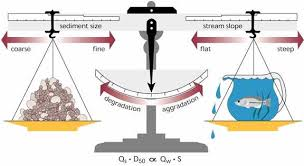
\includegraphics[scale=1]{immagini/bilancia_lane.jpg}
    \caption{Bilancia di Lane}
    \label{bilancia_lane}
\end{figure}
Matematicamente, il comportamento di un torrente al fine di ottenere l'equilibrio può essere riportato con questa formula:
\begin{equation}
    Q_L \cdot S \overset{=}{\propto} Q_S \cdot D_{50}
    \label{bilancia_lane}
\end{equation}
Dove:
\begin{itemize}
    \item $Q_L$ è la portata liquida del corso d'acqua;
    \item $S$ è la pendenza del thalweg;
    \item $Q_S$ indica la portata solida di sedimenti trasportata;
    \item $D_{50}$ indica il valore mediano della serie granulometrica rilevata nell'alveo.
\end{itemize}
La formula \ref{bilancia_lane} può anche essere considerata come se al primo membro fosse rappresentata la ``stream power" del fiume ed al secondo membro fosse riportato l'attrito al movimento.\\
Secondo la ``Classificazione di Horatiis" (1930), i tratti fluviali di montagna possono essere suddivisi in:
\begin{itemize}
    \item torrenti di trasporto: l'energia della corrente è tale da essere completamente impegnata nel trasporto di materiale solido a valle; il letto tende a non abbassarsi o ad alzarsi. Le opere progettate per questi tratti hanno l'obiettivo di trattenere il sedimento;
    \item torrenti di scavo: l'energia della corrente produce trasporto solido ed incisione del letto; il letto tende ad abbassarsi, generando una tendenza all'incisione verso monte. Le opere progettate per questi tratti hanno l'obiettivo di consolidare maggiormente i tratti dove l'opera di erosione ha una maggiore presenza.
\end{itemize}

\subsection{Briglie di consolidamento}
Mediante le briglie di consolidamento si vuole indurre il tratto di reticolo verso una pendenza di equilibrio dinamico del profilo ($i_c$) \ref{profilo_briglia_consolidamento}.\\
La pendenza $i_c$ equivale alla pendenza che è necessario assegnare ad un certo tratto fluviale, affinché si trovi nelle condizioni di mettere in mobilità una precisa quantità granulometrica di sedimento al fondo.\\
Le briglie di consolidamento possono essere di tipo longitudinale (per la stabilizzazione delle sponde) o di tipo trasversale (al fine di ridurre o controllare la pendenza longitudinale del profilo.)
In molti casi, se necessario, vengono erette in successione una serie di briglie di consolidamento.

\begin{figure}[H] \centering
    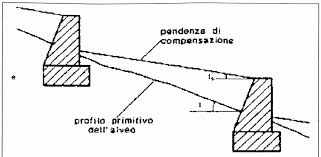
\includegraphics[scale=1]{immagini/profilo_briglia_consolidamento.jpg}
    \caption{Profilo di una briglia di consolidamento, con riportata la pendenza originaria e quella che si manifesta successivamente alla costruzione dell'opera.}
    \label{profilo_briglia_consolidamento}
\end{figure}

Il dimensionamento ed ulteriori informazioni su queste opere idrauliche verranno riportate più approfonditamente nel capitolo successivo.

\subsection{Studio della granulometria}
Con il termine ``granulometria" s'intende la proprietà con cui è possibile descrivere e studiare un insieme di particelle del suolo, siano queste sabbiose, ghiaiose,...\\
Lo studio granulometrico permette di conoscere, in modo statistico, la composizione del terreno di studio.\\
L'analisi granulometrica inizia andando a misurare, in modo sistematico, la grandezza (generalmente il diametro) dei clasti presenti nel letto dell'alveo o nelle barre.\\
Successivamente, si procede alla suddivisione in classi dei diametri misurati, per poi andare a calcolare la frequenza relativa, cumulata e percentuale per ognuna.\\
Per il caso di studio di questa relazione, la curva che interpola la frequenza cumulata e la classe diametrica dei sedimenti è la seguente.
\begin{figure}[H] \centering
    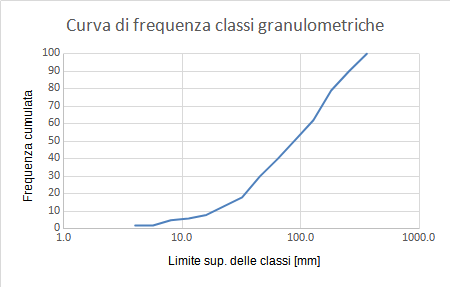
\includegraphics[scale=0.75]{immagini/curva_freq_classi_granuometriche.png}
    \caption{Curva della frequenza cumulata delle classi granulometriche.}
    \label{curva_freq_classi_granulometriche}
\end{figure}
Infine, per conoscere la distribuzione statistica delle grandezze dei  sedimenti, all'interno del campione rilevato, è necessario applicare la seguente formula:
\begin{equation}
D_\% = \left[\frac{D_2-D_1}{F_2-F_1}\right] \cdot (F-F_1)+D
\end{equation} 
Dove:
\begin{itemize}
    \item $D$ indica la classe diametrica;
    \item $F$ indica la frequenza cumulata.
\end{itemize}
Per il caso di studio inerente a questa relazione, i risultati sono:
\begin{table}[H]\centering
    \caption{\textcolor{red}{Classi di frequenza cumulata inerente ai sedimenti del bacino idrografico di studio. I valori relativi ai diametri sono espressi in $mm$.}}
    \begin{tabular}{cc}
    \toprule
    N   & 100      \\
    \midrule
    D16 & 28.25    \\
    D50 & 88.10    \\
    D84 & 215.10   \\
    D90 & 256.00   \\
    \bottomrule
    \end{tabular}
    \end{table}

\subsection{Calcolo della pendenza di correzione}
\subsubsection{Approccio statico per la stima di $i_c$}
Secondo Fattorelli et al. (1980), basandosi su 1000 tratti sistemati in Trentino, il valore $i_c$ può essere calcolato mediante le seguenti formule:
\begin{itemize}
    \item per bacini mediamente erodibili:
\begin{equation}
    i_c = 0.66 \cdot i_0 
\end{equation}
\item per bacini poco erodibili
\begin{equation}
    i_c = 0.77 \cdot i_0 
\end{equation}
\item per bacini molto erodibili
\begin{equation}
    i_c = 0.59 \cdot i_0 
\end{equation}
\end{itemize}
 
Secondo Heede (1960), il calcolo di $i_c$ avviene mediante:
\begin{equation}
    i_c = (0.6 - 0.7) \cdot i_0
\end{equation}

\subsubsection{Approccio mediante lo sforzo tangenziale medio}
Considerando le condizioni di moto uniforme ($i_F=i_E=i$), la corrente esercita sul contorno uno sforzo tangenziale medio, con formula:
\begin{equation}
    \tau = \gamma \cdot R_H \cdot i
\end{equation}
Conoscendo la $i_c$, ovvero la pendenza che si ambisce ad ottenere successivamente alla costruzione dell'opera, è possibile calcolare la $\tau_{c}$, mediante la formula precedentemente riportata.\\
Lo sforzo massimo che si genera nel letto del fiume, ha valore calcolabile mediante la formula:
\begin{equation}
    \tau_{max} = \gamma \cdot y \cdot i
\end{equation}
Mentre, per quanto riguarda lo sforzo agente sulle sponde, il calcolo avviene mediante:
\begin{equation}
    \tau_{sponde-fondo-max}= K \cdot (\gamma, y, i)
\end{equation}
Secondo le ricerche Shields (1936), e successive semplificazioni, la relazione tra sforzo al fondo e grandezza dei sedimenti è regolata dalla formula:
\begin{equation}
    \tau_c \approx 1000 \cdot D
    \label{tau_cr_shields}
\end{equation}
\subsubsection{Approccio deterministico per la stima di $i_c$}
Secondo Shields (1936), la formula per il calcolo dello sforzo tangenziale critico è:
\begin{equation}
    \tau_c = 0.06 \cdot (\gamma_s -\gamma) \cdot D
\end{equation}
Dove:
\begin{itemize}
   \item $D$ è la taglia granulometrica di riferimento;
    \item $\gamma_s$ è il peso specifico dei sedimenti;
    \item $\gamma$ è il peso specifico dell'acqua.
\end{itemize}
Tale formula può anche essere riscritta, diventando:
\begin{equation}
    i_c = \frac{\tau_c^* \cdot (\gamma_s-\gamma) \cdot D}{\gamma \cdot Rh}
\end{equation}

\subsubsection{Soluzione esplicita semplificata per sezioni rettangolari molto larghe}
Nel caso in cui il corso d'acqua dovesse passare attraverso una sezione rettangolare ampia e con un tirante idraulico ridotto, è possibile adottare alcune approssimazioni e semplificazioni.\\
Data una sezione rettangolare, potendo trascurare l'altezza del tirante idraulico $h$, il raggio idraulico $Rh$ risulta essere:
\begin{equation}
    \frac{B \cdot h}{B + 2\cdot h} \approx \frac{B \cdot h}{B} \approx h
\end{equation}
La formula per il calcolo del coefficiente di scabrezza $ks$, conoscendo il parametro relativo alla granulometria $D_{90}$ è:
\begin{equation}
K_s \approx \frac{26}{D_{90}^{1/6}}
\end{equation}
Essendo che la portata $Q$ è calcolabile come il prodotto dell'area per la velocità, è possibile esplicitare tutte e due le componenti della formula, che diventa:
\begin{equation}
    Q = (Ks \cdot Rh^{2/3} \cdot \sqrt{i_c}) \cdot (B \cdot h)
    \label{portata_sez_rett}
\end{equation}
Dove:
\begin{itemize}
    \item Ks è il coefficiente di scabrezza del fondo $\left[\frac{m^{1/3}}{s^{-1}}\right]$;
    \item Rh indica il raggio idraulico $[m]$;
    \item $i_c$ è la pendenza di correzione $\left[\frac{m}{m}\right]$;
    \item B è la larghezza dell'alveo $[m]$;
    \item h è la profondità del tirante idraulico $[m]$.
\end{itemize}
Sostituendo alla formula \ref{portata_sez_rett} il raggio idraulico, la formula diventa:
\begin{equation}
    Q = (Ks \cdot h^{2/3} \cdot \sqrt{i_c}) \cdot (B \cdot h)
\end{equation}
Che diventa:
\begin{equation}
    Q = (Ks \cdot h^{5/3} \cdot \sqrt{i_c}) \cdot B
\end{equation}

Il procedimento prosegue mediante il calcolo della pendenza di correzione:
\begin{equation}
    i_c = \left(\frac{0.1 \cdot D_{90} \cdot ks^{0.6} \cdot B^{0.6}}{Q^{0.6}_{30}} \right) ^{1.43}
    \label{pend_critica_iterativo}
\end{equation}
La profondità del tirante relativo alla condizione critica è calcolabile mediante la formula:
\begin{equation}
    h_c = \left( \frac{Q}{ks \cdot B \cdot \sqrt{i}}\right)^{3/5}
\end{equation}
Nel caso in cui il rapporto tra $h_c$ e $D_{84}$ è minore a 3.5, è possibile iniziare il procedimento di calcolo iterattivo mediante la formula di Barhurst (1985):
\begin{equation}
    Ks= \frac{\sqrt{g}}{h^{1/6}} \left[5.62 \cdot \log \left(\frac{h}{D_{84}}\right)+4\right]
\end{equation}
Dal valore di scabrezza calcolato è possibile ricavare il valore di pendenza critica, sempre mediante la formula \ref{pend_critica_iterativo}. Il procedimento iterativo termina quando il valore di scabrezza ks non si discosta molto da quello ricavato precedentemente.

\subsection{Determinazione di altezza e numero di briglie di consolidamento}
Successivamente ad aver calcolato la pendenza di correzione più ottimale per il caso di studio, è necessario valutare le misure di massima delle briglie, quali altezza, numero ed interdistanza tra ciascuna.\\
Come primo passaggio è necessario calcolare la variazione di quota totale per tutto il tratto, ed avviene mediante la formula:
\begin{equation}
    \Delta Z = (i_0 - i_c) \cdot L_s
\end{equation}
Successivamente, è necessario porre un'altezza di primo tentativo della briglia. Utilizzando questo valore per dividere la differenza di quota totale, è possibile calcolare il numero di opere in serie da costruire.\\
Infine, dividendo la distanza totale del tratto per il numero di opere da ereggere, si ricava l'interdistanza lineare tra una briglia e la successiva.

\subsection{Calcolo della pendenza di correzione per il tratto di studio}
Dopo aver descritto i vari procedimenti per il calcolo della pendenza di correzione, è possibile applicare i concetti per il caso di studio di questa relazione.\\
Dal programma GIS è possibile evidenziare il tratto di reticolo idrografico soggetto alla sistemazione idraulica mediante briglie.
\begin{figure}[H] \centering
    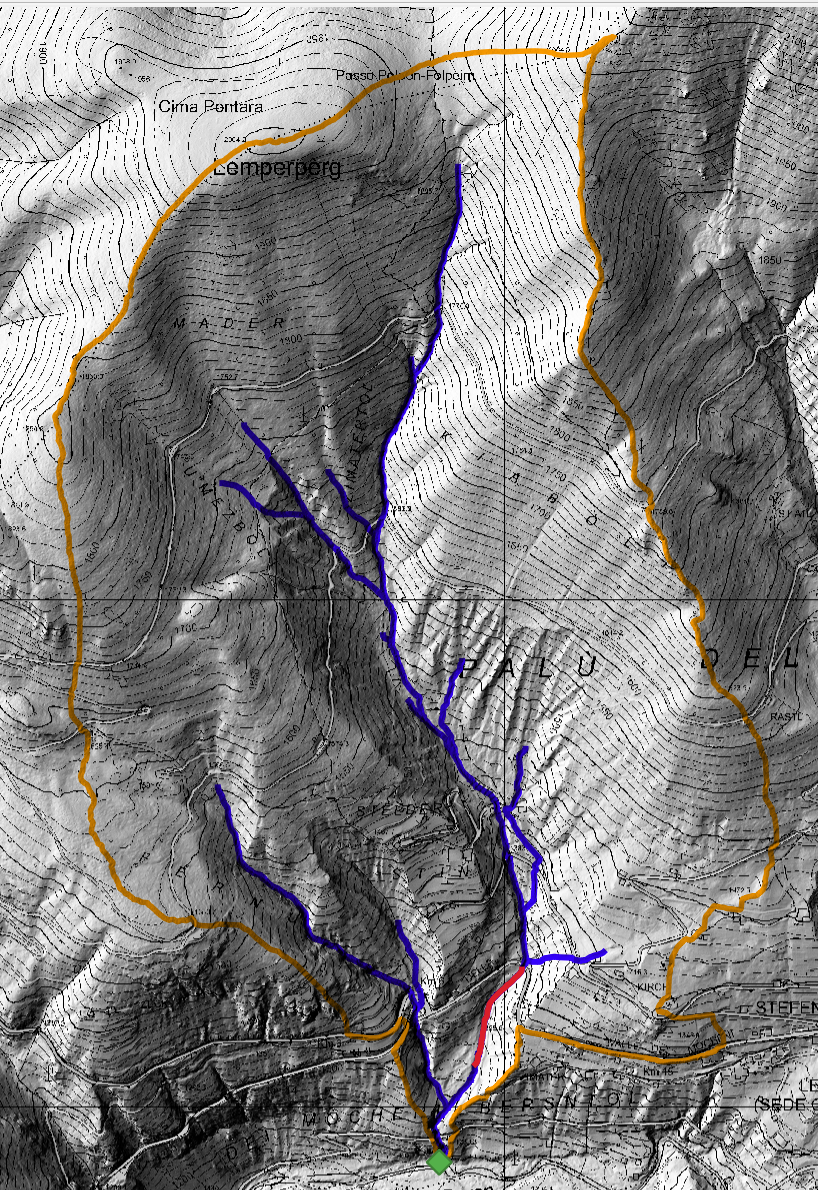
\includegraphics[scale=0.3]{immagini/pendenza_planimetria_1.png}
    \caption{Rappresentazione planimetrica del bacino di studio e del reticolo idrografico, con evidenziato in rosso il tratto interessato dalla sistemazione idraulica.}
    \label{pendenza_planimetria_1}
\end{figure}
\begin{figure}[H] \centering
    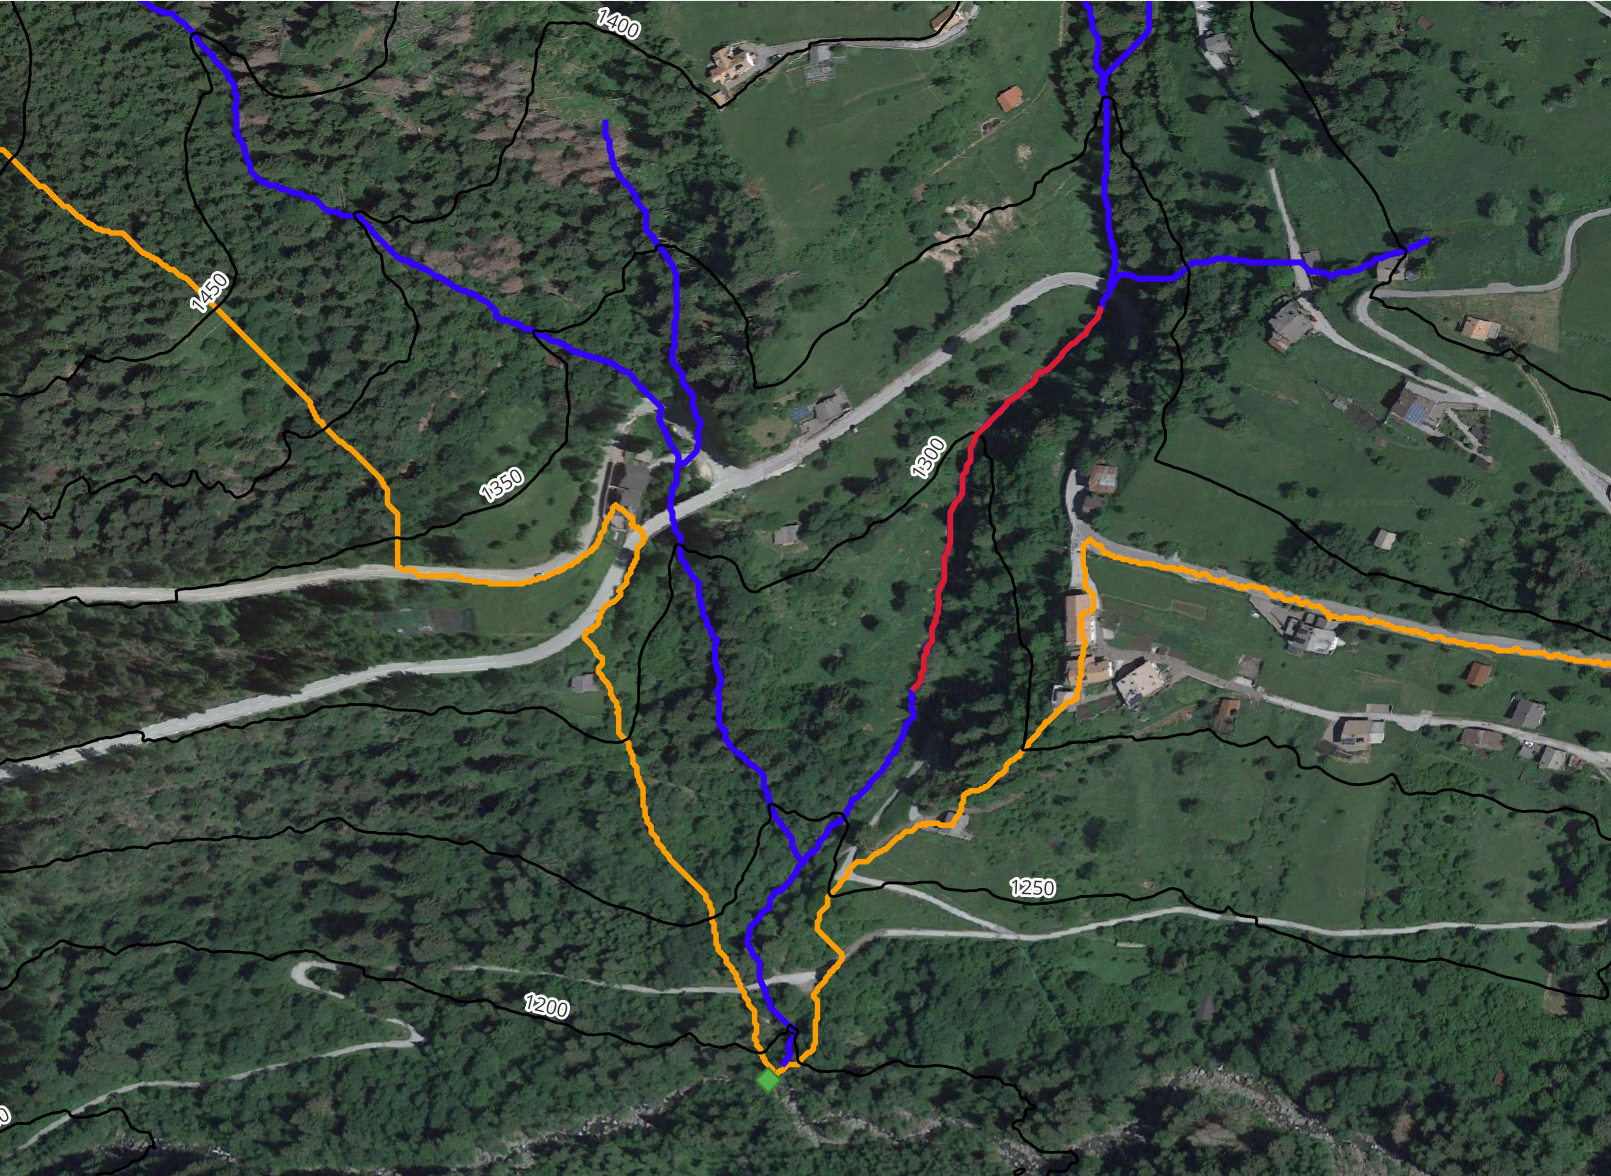
\includegraphics[scale=0.3]{immagini/pendenza_planimetria_2.png}
    \caption{Particolare del bacino di studio, con rappresentazione del tratto soggetto a sistemazione idraulica.}
    \label{pendenza_planimetria_2}
\end{figure}
\begin{figure}[H] \centering
    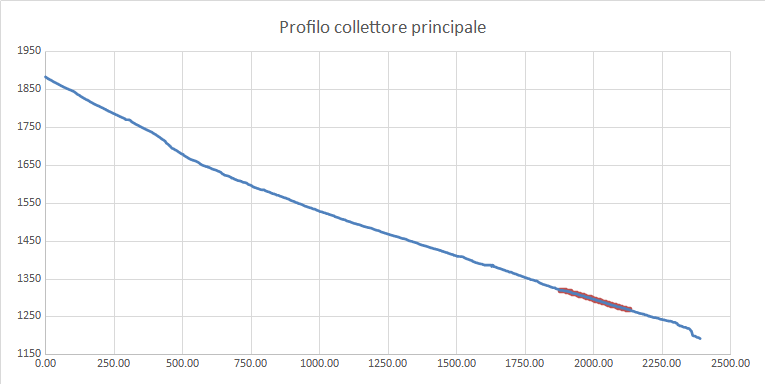
\includegraphics[scale=0.5]{immagini/pendenza_collettore.png}
    \caption{Rappresentazione del profilo del collettore principale, con indicazione del tratto soggetto a sistemazione idraulica (in rosso).}
    \label{pendenza_collettore}
\end{figure}
Mediante dei semplici passaggi matematici, svolti nel programma di calcolo, è possibile ricavarsi le principali informazioni morfologiche inerenti al tratto interessato da sistemazioni:
\begin{table}[H] \centering
    \caption{\textcolor{red}{Principali informazioni morfologiche inerenti al collettore principale del reticolo idrografico e del tratto interessato dalle sistemazioni.}}
    \begin{tabular}{ccc}
    \toprule
                 & collettore & tratto da sistemare \\
    \midrule
    lunghezza    & 2388.27    & 250.83              \\
    pendenza m/m & 0.29       & 0.20                \\
    pendenza °   & 16.12      & 11.57               \\
    \bottomrule
    \end{tabular}
\end{table}

Successivamente ad aver svolto per due volte i calcoli iterativi, al fine di ottenere i valori di scabrezza e di pendenza maggiormente ottimali, si è giunti ai seguenti risultati:
\begin{itemize}
    \item ks = 17.0 $\frac{m^{1/3}}{s}$;
    \item $i_c$ = 0.110 $\frac{m}{m}$.
\end{itemize}

Infine, si procede al calcolo del numero di opere in serie da ereggere e le relative interdistanze, imponendo l'altezza del livello inferiore della gaveta.\\
Vengono riportati alcuni risultati.
\begin{table}[H] \centering
    \caption{\textcolor{red}{Serie di risultati inerenti ai valori di numerosità ed interdistanza delle briglie, in funzione dell'altezza imposta.}}
    \begin{tabular}{ccc|ccc}
        \toprule
    Scenario 1 & $\Delta Z$ (m)& 23.68 & Scenario 4 & $\Delta Z$ (m) & 23.68 \\
& Z (m)         & 2.37  &            & Z (m)         & 3.40  \\
& n             & 10.0  &            & n             & 7.0   \\
& interdistanza & 25.11 &            & interdistanza & 36.02 \\
\midrule
Scenario 2 & $\Delta Z$ (m)        & 23.68 & Scenario 5 & $\Delta Z$ (m) & 23.68 \\
& Z (m)         & 3.95  &            & Z (m)         & 4.75  \\
& n             & 6.0   &            & n             & 5.0   \\
& interdistanza & 41.84 &            & interdistanza & 50.32 \\
    \midrule
Scenario 3 & $\Delta Z$ (m)        & 23.68 & Scenario 6 & $\Delta Z$ (m)        & 23.68 \\
& Z (m)         & 1.70  &            & Z (m)         & 2.62  \\
& n             & 13.9  &            & n             & 9.0   \\
& interdistanza & 18.01 &            & interdistanza & 27.75 \\
\bottomrule
\end{tabular}
\end{table}

\subsection{Calcolo preliminare del trasporto solido}
Shields (1936), grazie ai suoi studi effettuati sul trasporto solido, riuscì a ricavare empiricamente la formula dello sforzo tangenziale critico (necessario a muovere i sedimenti nel letto di un fiume), in funzione del peso specifico dell'acqua, dei sedimenti e della grandezza delle particelle granulometriche.\\
Tale formula, già riportata precedentemente, è \ref{tau_cr_shields}.\\
Da tale formula è possibile calcolare l'altezza del tirante idraulico che genera lo sforzo tangenziale in grado di muovere i sedimenti, conoscendo il peso volumetrico dell'acqua in movimento e della pendenza del corso:
\begin{equation}
    h_c = \frac{\tau_c}{\gamma \cdot i} 
\end{equation}
Mediante la conoscenza delle pendenze del tratto precedentemente e successivamente alla sistemazione, è possibile valutare come cambia il trasporto solido, calcolato mediante questo procedimento preliminare.\\

\begin{table}[H]
    \caption{\textcolor{red}{Trasporto solido di fondo, calcolato nelle condizioni precedenti e posteriori alla sistemazione idraulica del tratto di corso.}}
    \begin{tabular}{cccccccccc}
    \multicolumn{4}{l}{Situazione ANTE SISTEMAZIONE} &      & \multicolumn{4}{l}{Situazione POST SISTEMAZIONE} &      \\
    \textit{i0 =}  & 0.205  & \textbf{}  & \textbf{} &      & \textit{ic =}  & 0.110  & \textbf{}  & \textbf{} &      \\
                   &        &            &           &      &                &        &            &           &      \\
                   & D50    & D84        & D90       &      &                & D50    & D84        & D90       &      \\
                   & 0.089  & 0.215      & 0.256     & m    &                & 0.089  & 0.215      & 0.256     & m    \\
    $\tau_c$            & 89     & 215        & 256       & N/m2 & $\tau_c$       & 89     & 215        & 256       & N/m2 \\
    hc            & 0.04   & 0.11       & 0.13      & m    & hc         & 0.08   & 0.20       & 0.24      & m    \\
    Qc& 0.015  & 0.898      & 1.378     & m3/s & Qc & 0.32   & 2.71       & 3.90  & m3/s
    \end{tabular}
    \end{table}